\chapter{Implementation}
\label{chapter:implementation}

This chapter will go through the implementation of the project. First, the system information and general program structure will be looked at. Then, the rendering of fractals will be covered, followed by the attempts at improving performance, and the method of measuring performance. Finally, there will be a section on debugging.\newline

In terms of general optimizations, there were no specific efforts to optimize the code or the basic algorithms (except perhaps to implement a view distance limit), since the most important thing was to remain consistent across the different scenarios, and the relevant measurements were the performance differences (if any), not the raw performance.

\section{Operating System and Hardware}

The operating system used was Linux Mint 20.1. No other operating system was tested.\newline

The CPU used was an Intel\copyright Core$^{TM}$ i7-9750H with 6 cores.

The GPU used was an NVIDIA TU106M (GeForce RTX 2060 Mobile).

The Vulkan version being used was 1.3.205.

\section{Program Structure and Libraries}

\subsection{Build System}

The build system chosen was Make. The project is small in terms of the code base so writing a Makefile for compilation was simple. A shell script was also written, and run from Make, that used GLSLC to compile the shaders and place them in the appropriate directories. GLSLC is licensed under the Apache License Version 2.0 \cite{licensing-glslc}.

\subsection{Language and Libraries Used}

The programming language of choice for this project was C, because it is the language that the libraries used were written in, and it's simple and efficient.

\subsubsection{Vulkan}

Vulkan was chosen because it is performant and modern, and because there is a new feature on the way that will, I think, help with the efficiency of rendering using one of the optimization methods chosen (this will be mentioned in the Conclusion chapter). It is licensed under the Apache License 2.0 \cite{licensing-vulkan}.

\subsubsection{Volk}

The third-party library, Volk, is a meta-loader for Vulkan. It allows one to load the Vulkan API without needing to link to Vulkan. This makes setup much easier to manage. It is licensed under the MIT license \cite{licensing-volk}.

\subsubsection{GLFW}

GLFW is a library for creating windows and surfaces, which can be used for Vulkan development. Additionally, it is easy to use and multi-platform, so was the logical choice for this project. It is licensed under the zlib/libpng license \cite{licensing-glfw}.

\subsection{Vulkan Setup}

The rendering process was split into two passes, one for geometry and one for colour. This was done because the speed at which the geometry of the scene was obtained was of interest, and the speed of colouring the fractals was not, so splitting them enabled measurement of the geometry render pass on its own. No vertices are passed in to the shaders; the vertex shaders conjure up fullscreen triangles using the vertex indices, which are then worked on by the fragment shaders, where all the calculations and colouring happen.\newline

Specific setups for different optimization methods will be discussed in the relevant sections.

\subsection{Program Arguments and Controls}

The program takes arguments which specify the setup when the program is loaded. The user can change which fractal to display (including the 2D Mandelbrot set, the Mandelbulb and the Hall of Pillars), which optimization method to use, whether to vary any fractal parameters (which can be used to animate the fractal) and whether to take any performance measurements during runtime. Some of the arguments affect which shaders are loaded, and the Vulkan setup.\newline

The user is able to control the camera with the mouse and keyboard, speed up and slow down, and print the current position and camera front vector. Input is handled by GLFW.

\section{Rendering 3D Fractals}

The project made use of two fractal formulae. One was for the Mandelbulb, as described in the background section. Another was chosen to provide variety, specifically with regards to the depth of the image. The Mandelbulb is neatly contained within a box, and the program renders its exterior, but not any `interior'. The alternative fractal (named `Hall of Pillars' by me given its lack of another name) is reminiscent of a room with many archways, which I thought might give a greater variety of results in terms of the performance measurements when using the optimizations developed in the project.\newline

The calculations for the fractals were done entirely within shaders, except for the generation of the 3D signed distance field, which was calculated on the CPU upon loading the program, before any rendering occurred. Single-precision floating point numbers were used for all calculations within shaders. These were chosen over double-precision numbers, as the scale of the fractals was reasonable, and high-detail zooms into the fractal were not necessary for the project.

\subsection{Basic Sphere Tracing Implementation}

The basic sphere tracing algorithm was implemented in GLSL and is largely the same across the fractal types and optimization methods. Figure \ref{figure:glsl-sphere-tracing} shows the implementation.

\begin{figure}[ht]
	\centering
	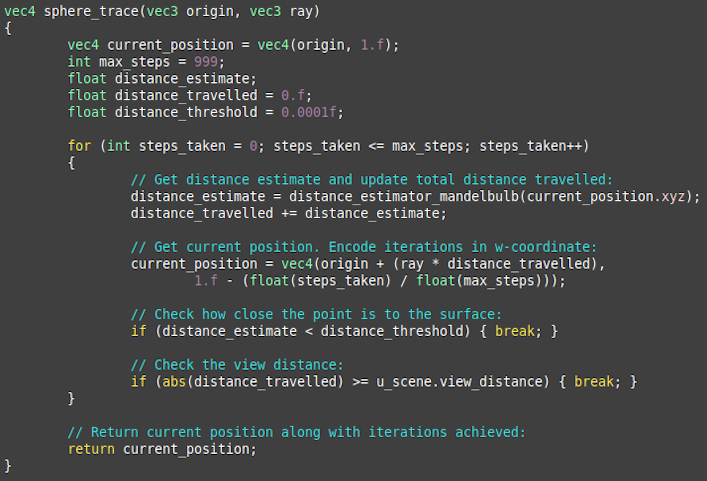
\includegraphics[width=0.65\linewidth, frame]{Images/GLSL-Sphere-Tracing.png}
	\caption{GLSL code snippet of the sphere tracing algorithm.}
	\label{figure:glsl-sphere-tracing}
\end{figure}

The most important things that must remain consistent between different optimizations on the same fractal are the termination conditions, which are as follows:

\begin{itemize}
	\item The maximum number of iterations allowed.
	\item The distance threshold.
	\item The view distance, contained in the scene uniform.
\end{itemize}

\subsection{Mandelbulb Fractal}

\begin{figure}[ht]
	\centering
	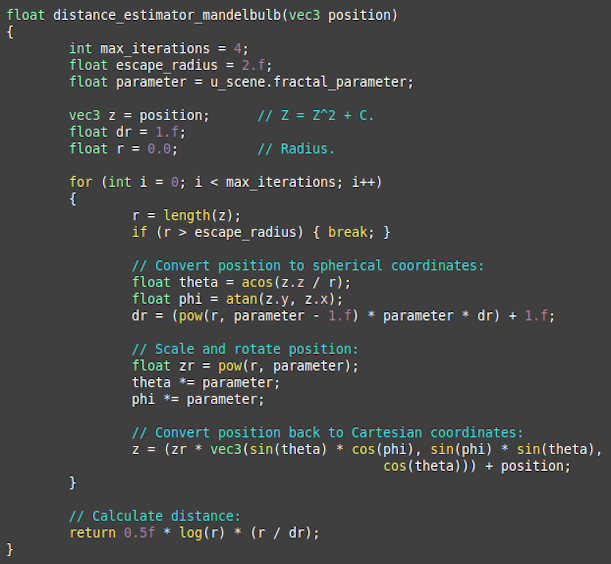
\includegraphics[width=0.65\linewidth, frame]{Images/GLSL-Distance-Estimator-Mandelbulb.png}
	\caption{GLSL code snippet of the distance estimator function for the Mandelbulb fractal.}
	\label{figure:glsl-distance-estimator-mandelbulb}
\end{figure}

\begin{figure}[ht]
	\centering
	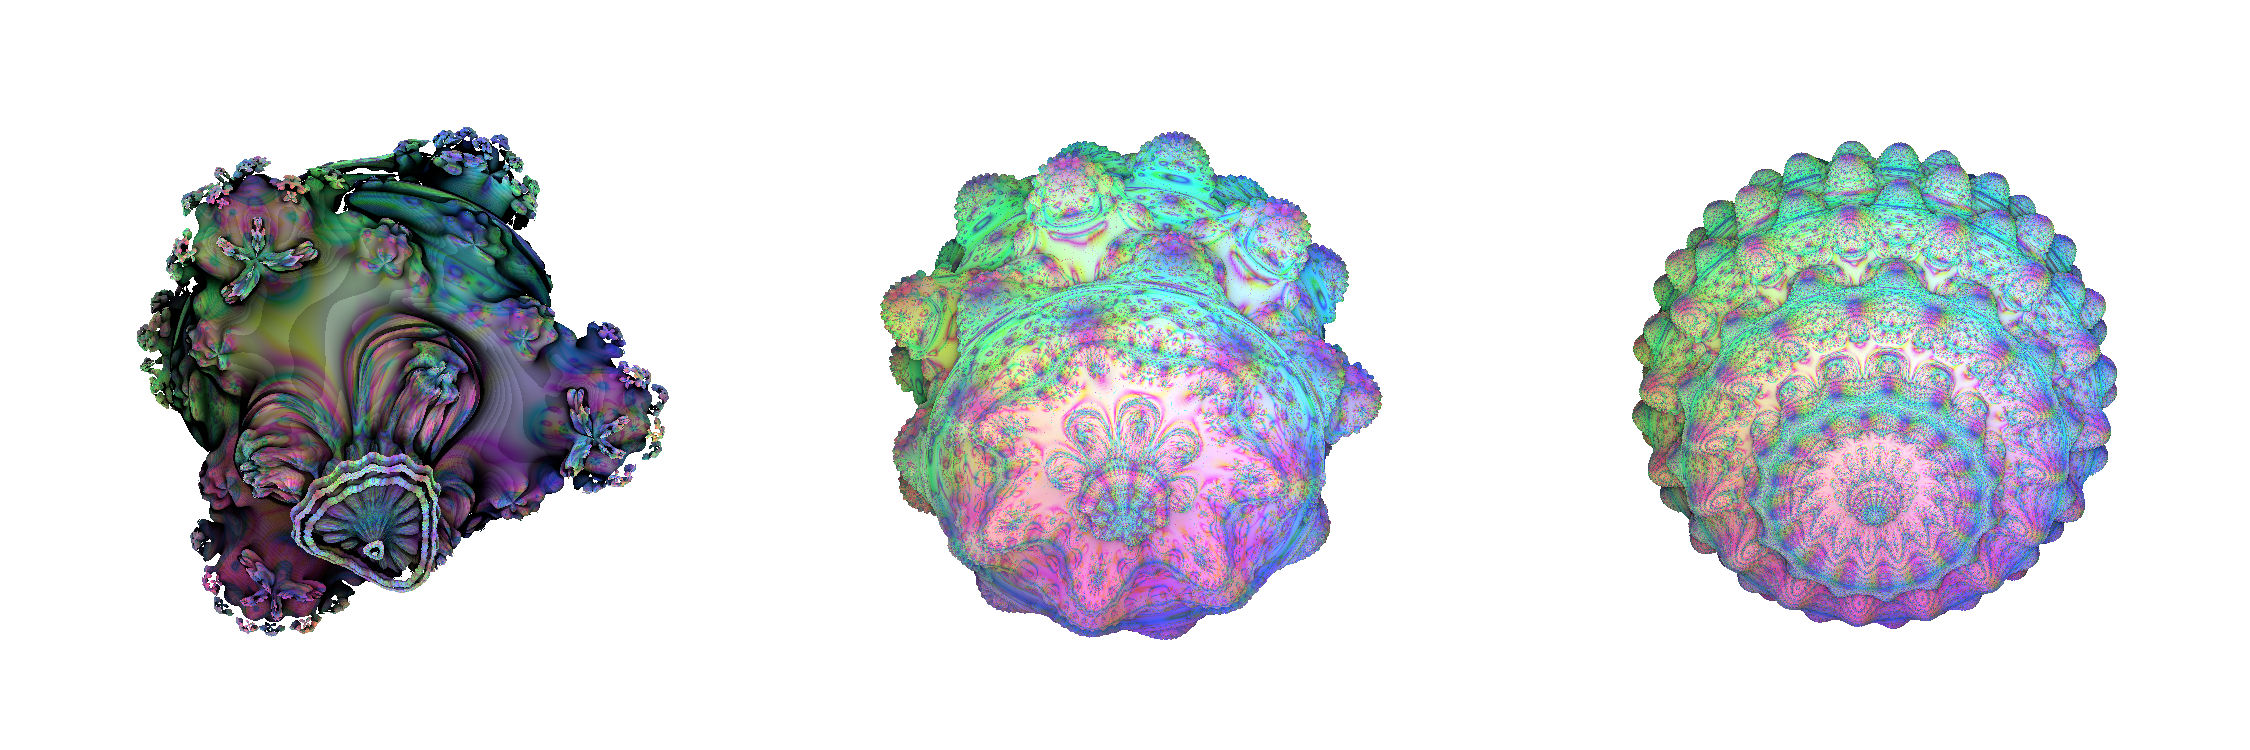
\includegraphics[width=0.65\linewidth, frame]{Images/Mandelbulb-Powers.png}
	\caption{The Mandelbulb, raised to different powers. Left to right: four, eight, sixteen.}
	\label{figure:mandelbulb-powers}
\end{figure}

Figure \ref{figure:glsl-distance-estimator-mandelbulb} shows the implementation of the distance estimator for the Mandelbulb fractal. Recall equations \ref{equation:mandelbulb} and \ref{equation:mandelbulb-power}. Equation \ref{equation:mandelbulb} is iterated over four times maximum. During the iterations, the current point is converted to spherical coordinates, scaled, and then converted back to Cartesian coordinates using equation \ref{equation:mandelbulb-power}. The distance formula based on equation \ref{equation:final-distance-estimate} is used to get the final result. The gradient of |f(Z)| is computed during the iterations (represented by dr in the shader).\newline

The fractal parameter in the scene uniform is the power that Z is raised to in the Mandelbulb formula. Varying this parameter results in different forms of the Mandelbulb. By default this parameter is eight, to match the original discovery by Paul Nylander. Figure \ref{figure:mandelbulb-powers} illustrates the effect of varying this parameter.

\subsection{Alternative Fractal}

\begin{figure}[ht]
	\centering
	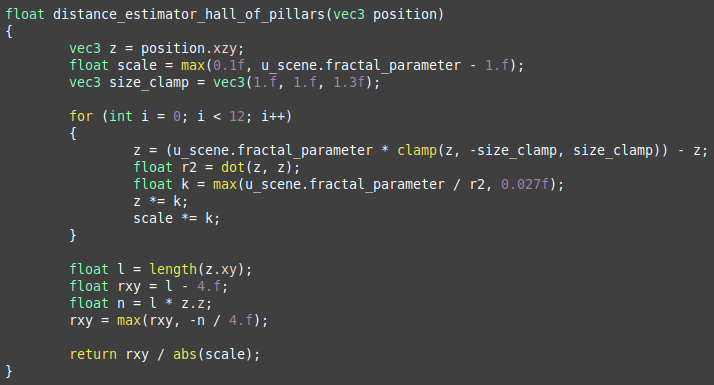
\includegraphics[width=0.65\linewidth, frame]{Images/GLSL-Distance-Estimator-Hall-Of-Pillars.png}
	\caption{GLSL code snippet of the distance estimator function for the Hall of Pillars fractal. Full credit goes to Dave Hoskins for the formula \cite{shadertoy-hall-of-pillars}.}
	\label{figure:glsl-distance-estimator-hall-of-pillars}
\end{figure}

\begin{figure}[ht]
	\centering
	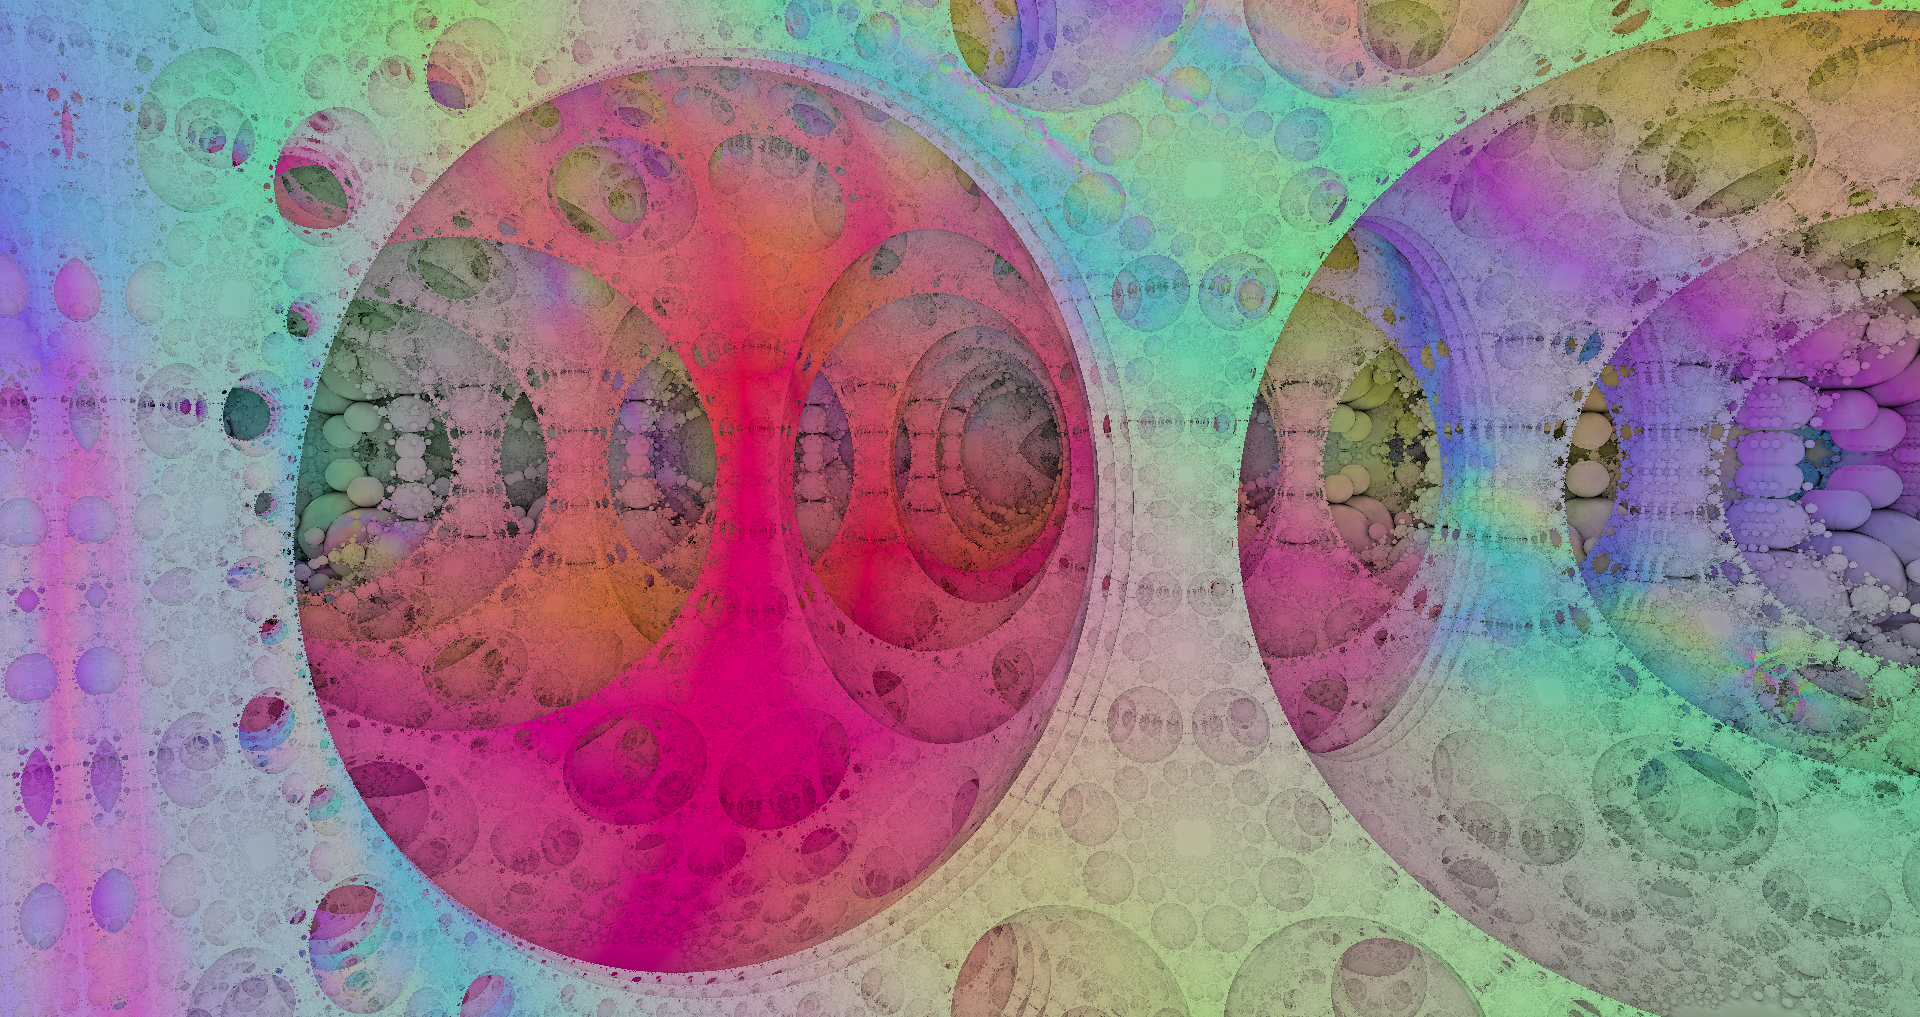
\includegraphics[width=0.65\linewidth, frame]{Images/Hall-Of-Pillars-Example.png}
	\caption{Rendering of the Hall of Pillars fractal.}
	\label{figure:hall-of-pillars-example}
\end{figure}

Figure \ref{figure:glsl-distance-estimator-hall-of-pillars} shows the implementation of the distance estimator for the alternative `Hall of Pillars' fractal. This fractal has different mathematical origins to the Mandelbulb, and is known as a Pseudo Kleinian fractal, but the mathematical background will not be explored here \cite{pseudo-kleinian-fractals}.\newline

As you can see from figure \ref{figure:hall-of-pillars-example}, this fractal varies a lot in depth, and  in particular has a lot of holes in it, so will result in the bottlenecks discussed in section \ref{section:temporal-caching}. The fractal formula was chosen for this reason, and to give variety when collecting results. Exploring the fractal also reveals large flat sections, and even larger `halls' much like the one in figure \ref{figure:hall-of-pillars-example}, as well as more intricate sections with great depth variety, but less overall depth. This fractal provided a good set of representative views for results collection.

\subsection{Colour}

Colour was not of the utmost importance in the project, so this section will be very brief. Colouring of the mandelbulb was done based on the closest distance from each point in the image to some fixed point. The Mandelbulb equation was iterated through, as in the distance estimation function, but in each iteration, the distance of the current point to a fixed point was measured, and the minimum of these was taken as a colour value.\newline

For the Hall of Pillars fractal, the colour was obtained in each iteration by getting the difference between elements of the current point and the previous point, and accumulating these differences.

\subsection{Ambient Occlusion}

\begin{figure}[ht]
	\centering
	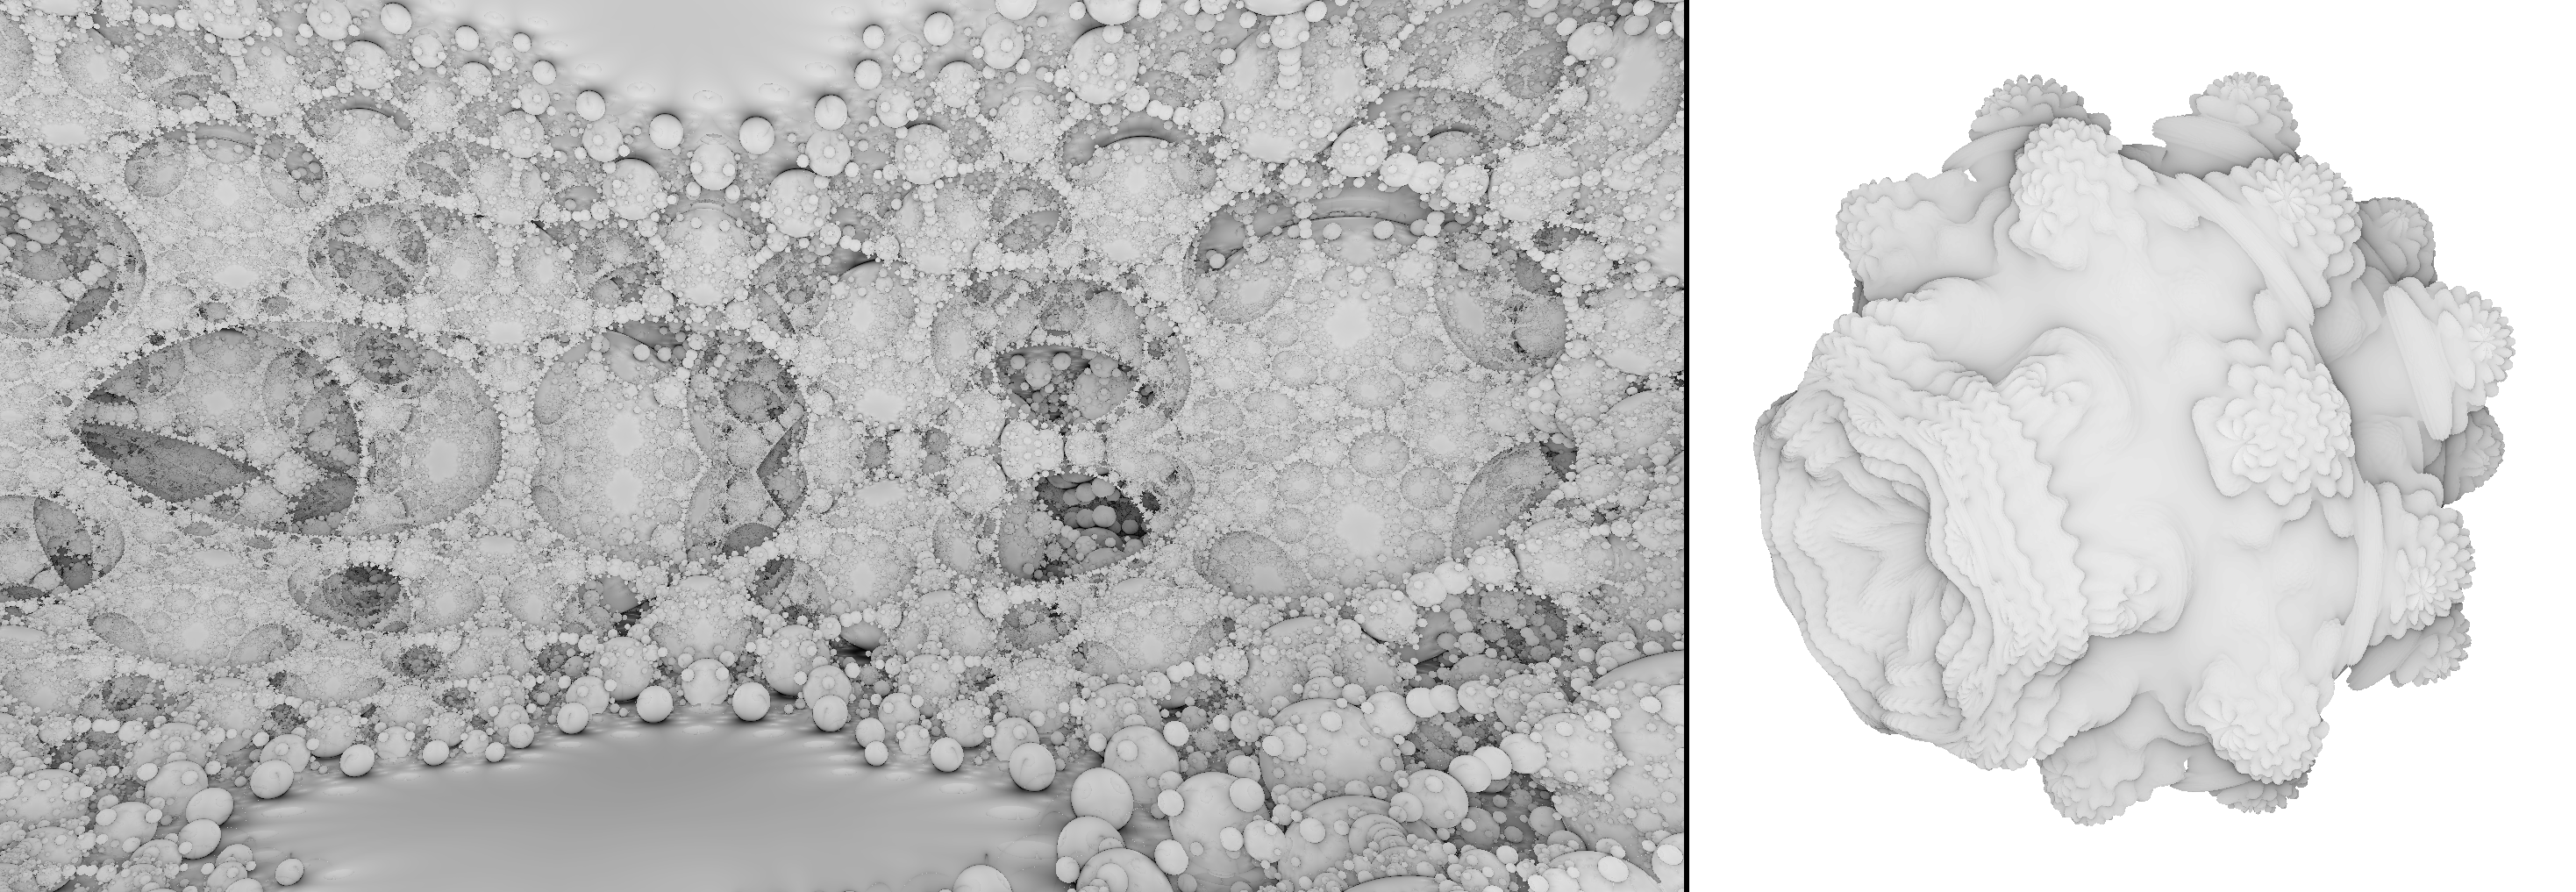
\includegraphics[width=\linewidth, frame]{Images/Ambient-Occlusion.png}
	\caption{Rendering of the Hall of Pillars fractal (left) and Mandelbulb (right), coloured based on the number of iterations achieved before reaching the surface.}
	\label{figure:ambient-occlusion}
\end{figure}

One of the consequences of using sphere tracing of signed distance functions is that it gives an estimate of the complexity of the surface. If a point takes more iterations to reach, then it's likely in a more complex area, and will be occluded. For both fractals in the project, the final colour is multiplied by a value between zero and one, based on the number of iterations achieved before reaching the surface. Figure \ref{figure:ambient-occlusion} shows renderings of the fractals used in this project, coloured purely based on the number of iterations.\newline

This free ambient occlusion effect also gives an informal measure of performance. Brighter areas mean less iterations, so two identical views can be compared which are using different optimization methods, to see if one performs better in terms of the number of iterations. Since this was the aim of using temporal caching, this was used as a measure of performance, in addition to render pass timings.

\section{3D Signed Distance Field}

\begin{figure}[ht]
	\centering
	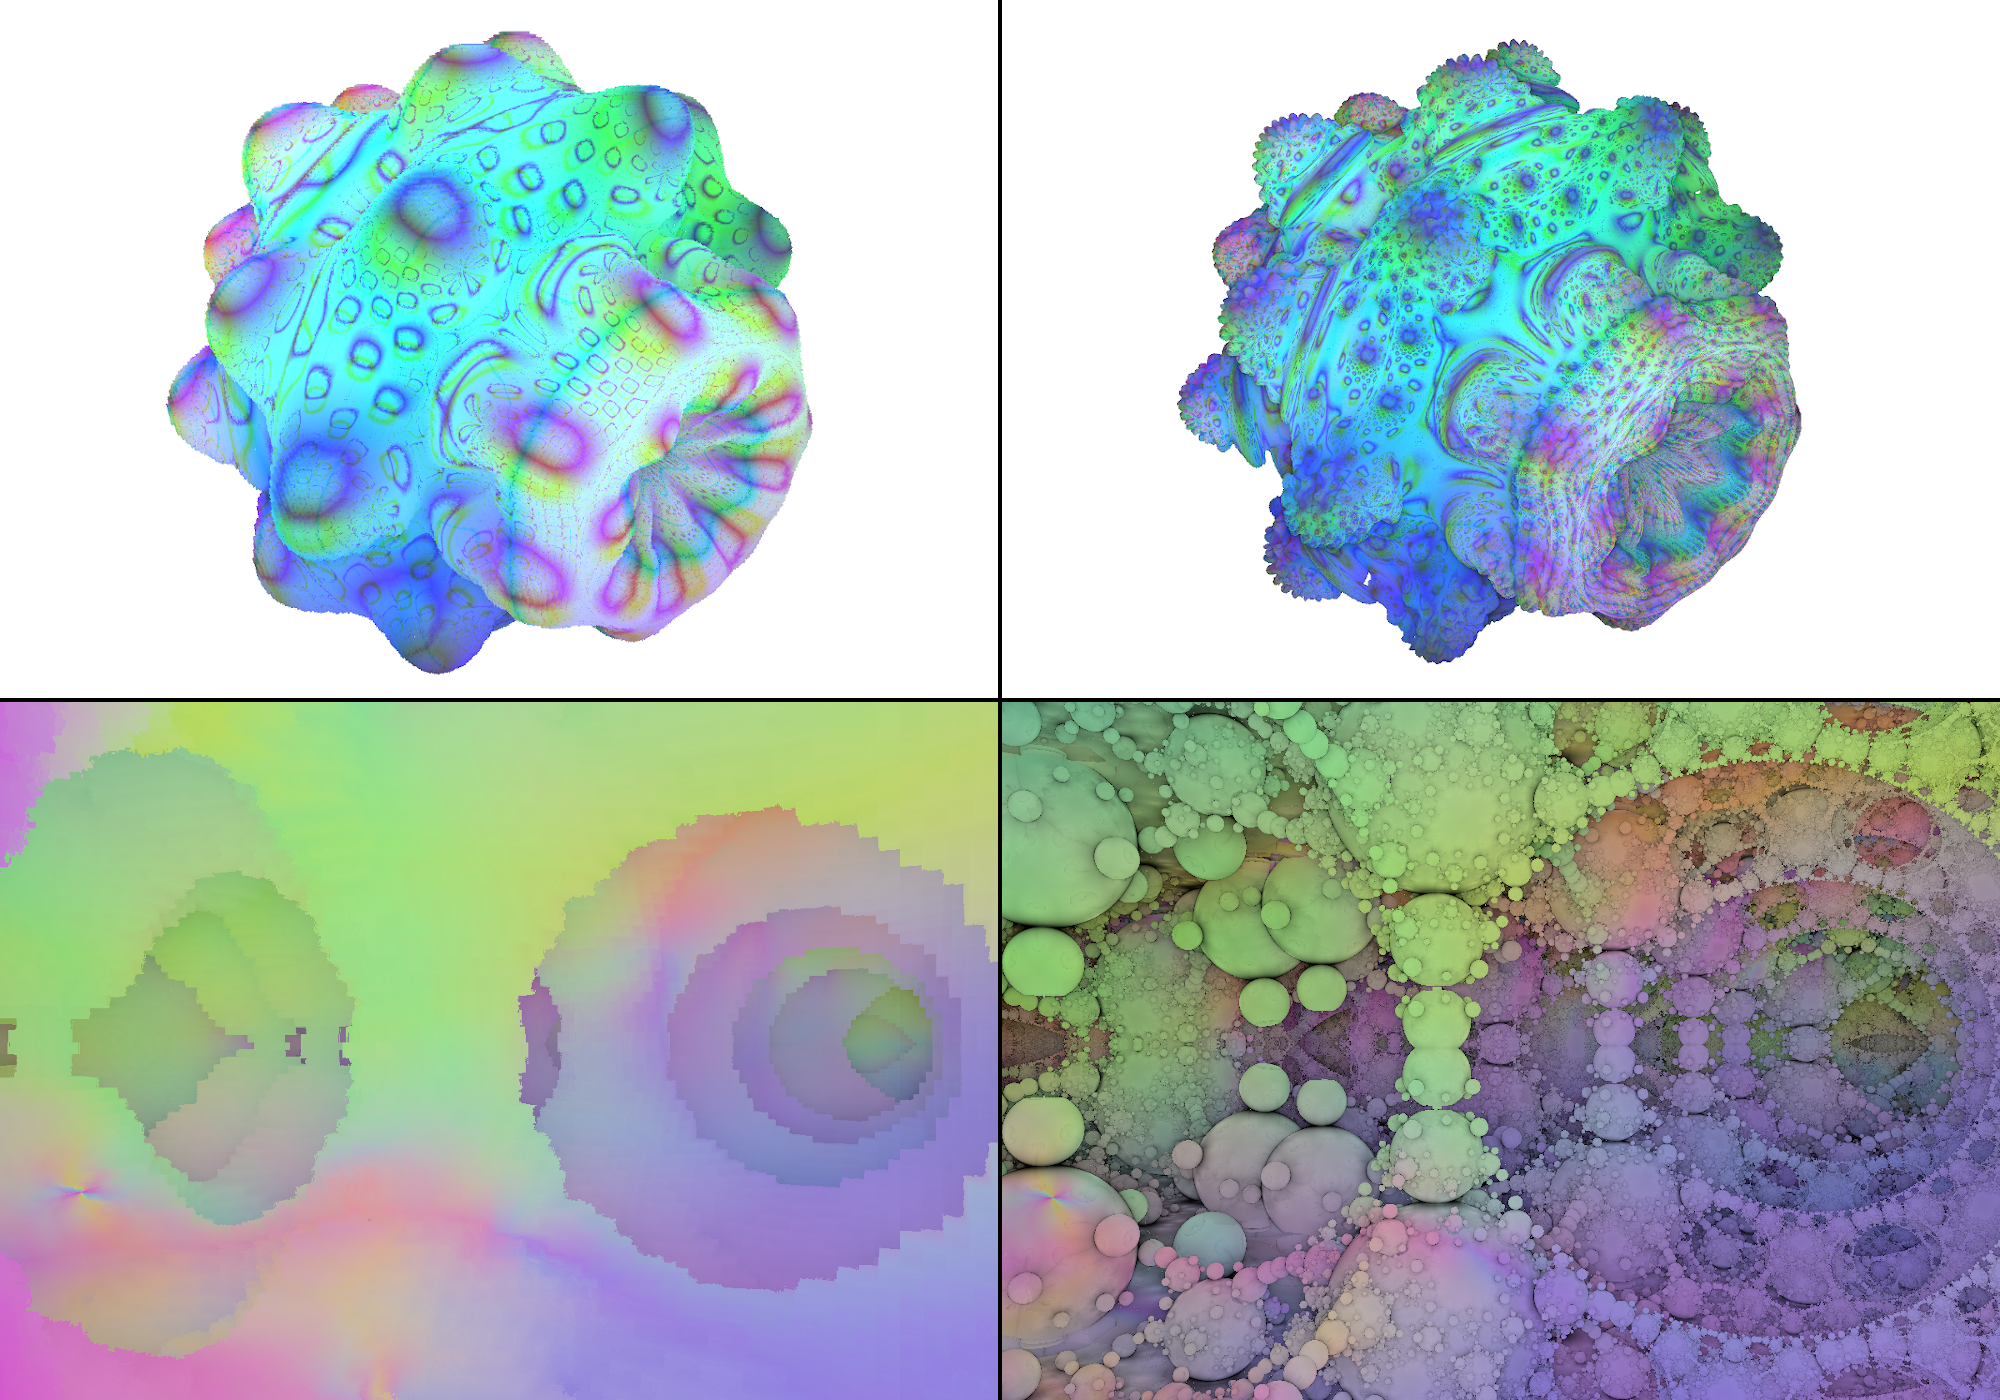
\includegraphics[width=0.65\linewidth, frame]{Images/SDF-Hybrid-Comparison.png}
	\caption{Rendering of the Mandelbulb (top) and Hall of Pillars fractal (bottom), using the signed distance field alone (left) and the hybrid approach (right). The Mandelbulb is rendered with 8 levels of subdivision (256$^3$ voxels), and the Hall of Pillars is rendered with 9 levels (512$^3$ voxels).}
	\label{figure:sdf-hybrid-comparison}
\end{figure}

\subsection{Structure and Usage}

The signed distance field represented a three-dimensional grid. Samples were taken at the centre of each voxel in the grid. To obtain a guaranteed underestimate here, the length of the line between the centre and corner of the voxel was taken away from this distance (or added, if the distance was negative). The more common approach is to sample the distance at the corners of the voxels and interpolate based on the location inside. The decision to only take the centre value was made to reduce memory reads, as the signed distance functions for the fractals are cheap in comparison to, say, the signed distance function for an arbitrary polyhedral shape.\newline

Another design decision that was made was to take a hybrid approach. Rather than try to obtain as much detail as possible (and use a lot of memory) in the signed distance field, the program performed sphere tracing through the field, until the sampled distance was smaller than the size of the diagonal between the voxel centre and corner; the largest distance possible from the centre before leaving the voxel. Obtaining a value such as this means that the surface is likely within the voxel. When this happens, the program reverts to using the signed distance function to obtain the finer detail. This provides a balance between speed, memory use and accuracy. Figure \ref{figure:sdf-hybrid-comparison} shows a comparison of visual quality for both fractals used in the project when using a signed distance field with the signed distance field alone, and using the hybrid approach.\newline

For the Hall of Pillars fractal particularly, the signed distance field does not have nearly the required level of detail, despite it having one more level of subdivision than the Mandelbulb. This is because this fractal has a much larger scale, so in order to cover a reasonable area of the fractal with the field, each voxel must be much larger. For the Mandelbulb, the whole shape can be contained in a small box, approximately 2.2 units along each edge. The Hall of Pillars fractal seems to be infinitely large. This difference makes the signed distance field very limited for use in large fractals.

\subsection{Octree Storage}

\begin{figure}[ht]
	\centering
	
\includegraphics[width=0.45\linewidth, frame]{Images/Octree-Structure.png}
	\caption{Structure of the signed distance field octree. Only child nodes of traversed nodes are shown.}
	\label{figure:octree-structure}
\end{figure}

\begin{figure}[ht]
	\centering
	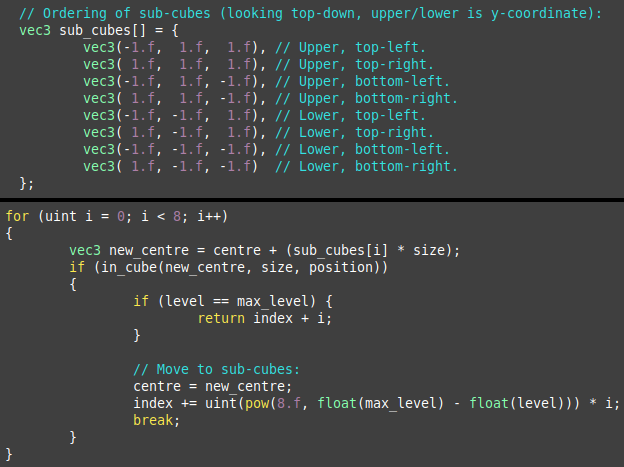
\includegraphics[width=0.65\linewidth, frame]{Images/Octree-Traversal.png}
	\caption{Code snippets from the octree traversal function. Only significant parts are shown.}
	\label{figure:octree-traversal}
\end{figure}

The signed distance field is represented as an octree. Figure \ref{figure:octree-structure} shows the layout. Only the leaf nodes hold data, and the higher level nodes aren't represented at all. The decision was made not to adaptively subdivide the tree to make a sparse layout. This is because it was desirable to reduce the number of memory reads, and instead calculate the index of the desired voxel by its depth and position inside the bottom level of the tree. This ruled out the use of adaptive sparse structures, as they would require more information on the subdivision of voxels, and so need to store information for higher-level voxels.\newline

The child nodes of every parent node are stored in the same order, which is what makes it possible to calculate the index without explicitly storing information about non-leaf voxels. In memory, the whole structure is represented as an array of floating point numbers; the calculated distances at the centre of each voxel. Additional, vital information is given in the scene uniform. This includes the size and centre of the root voxel, and the total number of subdivisions of the signed distance field. The values in the array are ordered left to right, as the leaf nodes would be if the whole tree was expanded.\newline

Figure \ref{figure:octree-traversal} shows a snippet of shader code for traversing the tree. No memory reads are required until the index of the leaf voxel is found (this function returns said index, which is used to fetch the data in the main sphere tracing function), so most of the effort is spent traversing the tree and calculating the index. This is in line with the goal of introducing as few memory reads as possible, since they are comparatively slow. As mentioned, for an arbitrary, complex polyhedral shape, this might not be a problem, but the fractals are fairly efficient to calculate, so the signed distance field traversal needs to be competitive, even at the expense of accuracy (hence the hybrid approach mentioned above).\newline

The calculation of the voxel index is based on its current level in the tree, compared to the maximum level, and its current position in the group of eight child voxels (see the lower image in figure \ref{figure:octree-traversal}). The centre positions of each voxel are calculated based on the position in the group of child voxels (the index of the loop is used to get a value from the array of positions, seen in the top of figure \ref{figure:octree-traversal}), and the current voxel size, which begins equal to the total signed distance field size, and is halved upon entering each new level.\newline

A further explanation on the calculation of the index will be given. Refer to figure \ref{figure:octree-structure}. The index of the current voxel begins at 0, which corresponds to taking the leftmost path until a leaf node is reached. In this case, the third voxel in the first level after the root is taken. This means that the index must be incremented by the number of leaf voxels that come before the leftmost path possible following this third voxel. Each voxel before this one has 8 child nodes, giving 8 * 2 = 16 nodes. Each of those 16 nodes divides into 8 as well, giving 16 * 8 = 128 leaf nodes that have been skipped. To calculate this, one must look at the number of levels left before the leaf level is reached. This is 3 - 1; the maximum level, which is 3, minus the current level, which is 1. This means that there are 2 subdivisions, which matches the amount counted when traversing the tree. Then, one must see how many nodes come before the current node, in the current level. This is equal to the current index, which is 2 (beginning at 0). This matches what is seen here. All that needs to be done now is calculating the number of leaf nodes. This is done by multiplying the number of previous nodes on the current level by the number of leaf nodes each one contains. This is 2 * 8$^2$ = 128, as expected.

\section{Temporal Caching}

\subsection{Data to Cache}

The data chosen to persist across frames was the true distance travelled by the ray. The aim of this optimization method was to reduce the number of iterations in certain areas of the image, especially edges and holes, so just storing the first distance estimate was not the solution. In order to preserve depth data for multiple frames, a texture image with red, green, blue and alpha floating-point components was chosen. With this, the data for the last four frames was stored.\newline

Alternative data was experimented with as well, such as end position, end distance estimate and the first distance estimate along the ray that was below a certain threshold. The end position was intended to help reveal if the end pixel location had moved too much, invalidating the data. To do this, the stored estimate was used to march the point along the ray for the current frame. The magnitude of the difference between the end position for the last and current frames was then used to determine validity. The end distance estimate was used for the same purpose, but allowed data to be stored for two previous frames, as opposed to just one. The reasoning behind only using one texture image was that sampling a texture requires an overhead that quickly builds up, so storing too much data may offset any performance benefit.\newline

The first distance estimate along the ray was intended to help determine if the current ray was close to an edge. As mentioned in section \ref{section:temporal-caching}, if some geometry occluded the ray, and the distance stored was greater than the distance to that geometry, artefacts would appear. A test was performed that would determine the risk that this had happened, based on the stored distance to an edge.\newline

In the end, storing the true distance travelled for the last four frames was the most effective in terms of performance and artefacts.

\subsection{Image Sampling}

The distance values were written to the G-Buffer for the first render pass. Every frame, the values were shifted one place to the right, discarding the last (alpha) value each time, and the new value was written to the first slot. After the render pass, the G-Buffer image was the copied over to a texture image, ready for sampling from during the next frame. Each pixel only sampled from its own position in the texture. It could be possible to do a kind of edge detection based on the depth values in neighbouring pixels, but this was deemed too expensive.

\subsection{Camera Movement}

\begin{figure}[ht]
	\centering
	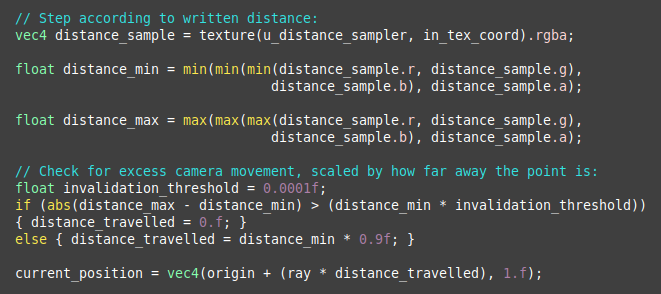
\includegraphics[width=0.65\linewidth, frame]{Images/Distance-Test.png}
	\caption{Test to determine if a pixel is invalid and the ray needs recasting.}
	\label{figure:distance-test}
\end{figure}

The test to see if the camera had moved too much is shown in figure \ref{figure:distance-test}. It relied on the difference between the largest distance sample and the smallest. Generally speaking, the `landscape' of the fractals chosen is not smooth, so this proved to be a reliable test for invalidated geometry, without triggering at the smallest movement. If the test passed, and the pixel was still valid, the minimum sampled distance estimate was chosen and reduced a little, to provide a reliable underestimate of the true distance for the current frame. The usual sphere tracing algorithm was then performed, using this head-start.

\subsection{Artefacts}

\begin{figure}[ht]
	\centering
	\includegraphics[width=0.65\linewidth, frame]{Images/Hall-Of-Pillars-Artefacts.png}
	\caption{Artefacts generated in a render of the Hall of Pillars fractal, by slow sideways movement, at different pixel invalidation thresholds.}
	\label{figure:hall-of-pillars-artefacts}
\end{figure}

The method for determining pixel invalidity was, unfortunately, not perfect. A balance had to be struck between maintaining a performance boost during camera movement, and reducing artefacts associated with overshooting the true distance. Particularly, since the method chosen relied on the fractal landscape changing in depth, when there were particularly smooth sections (such as when rays were hitting the view distance threshold), more artefacts appeared. Changing the threshold at which pixels are declared invalid can be done to balance artefacts and performance. Figure \ref{figure:hall-of-pillars-artefacts} shows how the severity of the artefacts varies with this threshold. It ranges from near-perfect (bottom image) to unacceptable degeneration of the scene (top image).\newline

The artefacts in figure \ref{figure:hall-of-pillars-artefacts} were triggered by slow, sideways movement and no camera rotation. The scene was chosen because of the large portion that was outside the allowed view distance, the presence of flat areas within view range, and the large number of edges at different view distances. The value for the threshold settled on was 0.0001, as shown in the centre image. This image represents a worst-case scenario for this particular scene at the different thresholds. The movement employed to get these artefacts to appear was rather specific, and unnatural for a lot of use cases, such as a game or fractal exploration animation. This is why the threshold chosen was deemed acceptable for use in this project. Any more relaxed and artefacts began to appear during more `natural' movement. Any less relaxed, and the performance benefits were lost during any sort of movement.

\section{Performance Measurement}

This section will go over how performance differences were measured, and how different scenarios were captured.

\subsection{Preparation for Data Collection}

In order to make sure the data collected was consistent, the following measures were taken:

\begin{itemize}
	\item Wait 1000 frames before starting any measurements, to give the GPU time to `warm up'.
	\item For static images, take measurements for 1000 frames, then choose data based on the whole set, such as median.
	\item For animated images, run the animation 25 times, then take measurements over sets of matching frames. 25 was chosen because the animations are of considerable length; the longest would have taken approximately 5 hours to run 100 times, but the chosen 1.25 hours was tolerable.
	\item Close all other running programs to minimize interrupts.
	\item Turn off the screensaver.
	\item Make all measurements at the same image resolution: 1280 by 720.
\end{itemize}

\subsection{Data Types Collected}

The main value taken to measure performance was the execution time of the geometry render pass. To accomplish this, a Vulkan query pool was used to collect timestamps at two different stages each frame. One stage was at the beginning of the render pass and one was at the end, in order to make sure the timestamps were taken at the correct times (Vulkan commands in a command buffer may execute in any order unless specific synchronization is added), and consistently, with flags specifying the pipeline stages at which to take the measurements.\newline

Measurements of static scenes were gathered over a total of one thousand frames before being written out to file. This was to reduce the likelihood of outliers in the data. The median value of the data was taken, as it reliably cuts out outliers and represents a sort of `average case'.\newline

The time it took to copy the image after the render pass was not included in the measurements, because copying the image could have been avoided by swapping the G-Buffer image and texture image after the render pass.

\subsection{Representative Views}

In order to obtain a useful set of data for performance differences, a set of representative views was chosen. They were selected to provide variety in the complexity of the scene, to see if either of the optimization methods chosen performed better under certain circumstances than in others. For example, the temporal caching method was theorized to give the most benefit in situations where there are a lot of holes and edges in the scene, so views were chosen to represent best and worst case scenarios for this theory.\newline

The views will be displayed in chapter \ref{chapter:results}, next to the data collected for each one, so the two can be looked at together.

\subsection{Animation}

As well as static scenes, animated scenes were created. For the Hall of Pillars fractal, a fly-through of the scene was created, varying the speed of the camera. This was intended to test the performance of the temporal caching method during movement of the camera, to see if there was still a benefit to using it while moving under different circumstances. Camera movement did not affect the signed distance field, so an animation was not created. Additionally since the range of the signed distance field was so small (especially for the Hall of Pillars fractal), an animation would have been rather limited.\newline

The other type of animation was accomplished by varying a parameter used in the calculation of the distance function for each fractal, which resulted in smooth changes in geometry. This was done for both fractals. This type of animation was not done for the signed distance field optimization method, since any change in the geometry invalided the data that had been calculated.

\section{Debugging}

Debugging for this project was done manually by printing information out to the terminal. There is a function to print out all values, including handles, for the program's Vulkan structures, to check that they have been initialized properly and to track any Vulkan errors.\newline

To debug the three-dimensional SDF, there is a function to print a subset of the voxels, to check that the search process works properly and that the voxels are stored in the correct order and with the expected range of values.\newline

The key to print the current position and camera front came in useful for checking camera movement, as well as creating animations.\newline

I also used Valgrind to search for and fix any errors with memory management. Unfortunately, it seems that either Vulkan or Volk causes some memory leaks, so debugging this was tricky. I commented out all functions to do with Vulkan (which, admittedly, is most of the program), and there were no leaks or errors. I uncommented only the function that initializes Volk, and it introduced memory leaks.\newline

I debugged the shaders by adding special return values at various locations, so that if there was a problem or a statement was not running when it should have been, the rendered image would not be as expected (for example, it may be entirely black). This was used in combination with RenderDoc to view the different render passes and pipeline stages.
